%!TEX root = ../TFM.tex

\section{La Gamificación}


\coment{Esto es lo que correspondería al marco teórico.}


En esta sección procedemos a describir en términos generales la Gamificación como estrategia metodológica.
%
Primeramente trataremos de clarificar el concepto de gamificación, porqué y cómo se puede gamificar un contexto.
%
Una vez detallado, en la siguiente sección trataremos de aplicar la gamificación en la educación.


La palabra \textit{Gamificación} es una traducción del término inglés \textit{Gamification}, palabra derivada del sustantivo \textit{game}.
%
En castellano no podemos considerar Gamificación como palabra derivada de otro sustantivo. 
%
Otra posible traducción sería ludificación, palabra derivada del adjetivo lúdico.
%
En este sentido podríamos utilizar la denominación ludificación, pero se ha preferido utilizar en esta tesis el término Gamificación para buscar la congruencia con la tendencia entre el profesorado.


\coment{Qué es la Gamificación}


Atendiendo a \cite{GamificationDef} podemos definir \concept{Gamificación} como \textit{el uso de elementos de juegos en contextos no lúdicos}. 

Esta definición no está restringida al ámbito educativo. 
%
De hecho, la Gamificación entendida como una estrategia o metodología es aplicada a día de hoy en diversos ámbitos. 
%
Por ejemplo, es una técnica muy utilizada en el campo del Marketing \cite{GamifyMark} y de los Recursos Humanos \cite{GamifyHR}.
%
Tanto la Educación, como los Recursos Humanos como el Marketing son contextos no lúdicos en los que al introducir de elementos de juegos estaríamos gamificando. 
%
Pero, ¿qué entendemos por elementos de juegos? 
%
Aquellas dinámicas, mecánicas y componentes que hacen atractivos los juegos.
%
Es importante clarificar que el término juegos engloba tanto juegos de mesa como videojuegos y juegos espontáneos.
%
Además, no todos los juegos tienen los mismos elementos.
%
Algunos juegos, por sus características, utilizan más unos determinados elementos que otros.
%
Con fines didácticos vamos a describir algunos de esos elementos, aunque más adelante se ofrecerá una lista más completa.

Por ejemplo, en los juegos se produce un feedback instantáneo: el jugador avanza un número de casillas, obtiene dinero al pasar por una casilla determinada, aparecen carteles con información sobre el desempeño (¡Sigue así!), etc.
%
Este feedback instantáneo no se produce en contextos no lúdicos.
%
Un trabajador de una empresa es evaluado (como mucho) una vez al año. 
%
¿Y si cada día recibiera un pequeño feedback sobre su rendimiento?


Otro elemento importante de algunos juegos es la posibilidad de tomar decisiones importantes.
%
De hecho, algunos juegos van modificando la historia del juego en función de las decisiones que va tomando el jugador. 
%
Esto ocurre en videojuegos (la saga Mass Effect sería un ejemplo) pero también en los tradicionales juegos de rol (Dragones y Mazmorras).
%
¿Trabajarán mejor los empleados de una empresa si los empleados pueden elegir en qué trabajar?
%
Algunos grandes proyectos de Google, como Gmail, han surgido como resultado del porcentaje de tiempo que la empresa establece para que sus trabajadores trabajen en sus propias ideas.

Imaginemos la siguiente situación: un consumidor puede elegir entre 2 fruterías con la misma variedad de frutas y precios similares.
%
Si en una de ellas cada semana hay una nueva oferta para un tipo de fruta específico y se anuncia como \textit{la fruta de la semana}, podría despertar atracción en el consumidor. 
%
Incluso podría ocurrir que el consumidor espere ansioso que comience una nueva semana para ver cuál es la nueva oferta de la frutería.
%
A este fenómeno se le denomina \concept[Bucle de atracción]{bucle de atracción}. 
%
Es muy típico en los videojuegos online que existan misiones diarias, misiones semanales e incluso eventos especiales en fechas especiales como podría ser Navidad o Primavera.
%
¿Mejoraría la motivación de los estudiantes de una asignatura que el profesor planteara un reto opcional cada semana y en fechas especiales?


\coment{Por qué gamificar}

\paragraph{¿Por qué gamificar?} Se han dejado algunas preguntas en el aire, pero todas ellas se pueden englobar en la siguiente pregunta: ¿La Gamificación en un determinado contexto concreto mejora el rendimiento de las personas en ese contexto?
%
Hay bastantes investigaciones recientes que intentan contestar a esta pregunta.
%
Recurriendo a una revisión bibliográfica \cite{EmpiricalGamification} encontramos que la mayoría de experimentos empíricos sobre Gamificación han tenido efectos positivos en términos motivacionales.
%
Sin embargo, no todos los estudios encontraron efectos positivos en todos los participantes.
%
Además, parece que la gamificación falla a largo plazo, tal vez por el efecto de la novedad. 
%
\footnote{Estos posibles peligros y otros se tratarán más adecuadamente en \ref{PosiblesPeligros}, cuando el lector disponga de visión más global de la gamificación.}

Pero la gamificación puede producir efectos beneficiosos más allá de la motivación.
% 
De acuerdo con \cite{kwerb-WhyGamify} la Gamificación permite fidelizar a las persona, hacer todavía más social el contexto, ofrecer a la persona un sentido del progreso en ese contexto y crear un hábito.


\subsection{Diferencias entre Juegos serios y Gamificación}

Es importante distinguir gamificación de juegos serios. Los \concept[Juegos serios]{juegos serios} consisten en la modificación del contexto transformándolo en un contexto lúdico, mientras que la gamificación incorpora elementos en un contexto no lúdico, manteniendo el contexto como no lúdico.
%
Un ejemplo de juego serio sería idear un juego de conquistas como el Risk para trabajar los mapas políticos con los alumnos. 

Aunque los juegos serios tengan consecuencias positivas y puedan ser una buena herramienta\footnote{Tanto es así que \cite{MetaSerious} concluye en su revisión que los juegos serios son más efectivos en contextos de aprendizaje pero menos efectivo que los métodos convencionales en términos motivacionales.}, su estudio se sale de esta tesis.

\subsection{Aspectos de la Gamificación}

\paragraph{Diseño enfocado en la persona:} 
Un contexto gamificado crea una experiencia.
%
La gamificación es \textit{human-focused design} en contraposición con \textit{function-focused design} \cite{BeyondPBL}.
%
La situación se transforma en una experiencia para el usuario, y esta es una de las claves.

Aunque pueda ser una obviedad, en un juego hay jugadores. No son tratados como participantes ni como usuarios, sino como jugadores.
%
Pensar en las personas participantes de un contexto que se quiere gamificar como jugadores es un paso importante.
%
Sitúa a esas personas como los protagonistas y como el centro de la experiencia, pues para eso están diseñados los juegos.
%
Además, los jugadores tienen un cierto sentido de autonomía y control sobre la experiencia.
%
Otra clave a considerar es la siguiente: un juego tiene la meta de que sus jugadores empiecen a jugar, frente a otras posibilidades a su alcance, y se mantengan jugando.
%
Una manera de conseguir esta meta es hacer el recorrido del juego o la experiencia gamificada con una dificultad que se incremente progresivamente y de acuerdo a lo que el jugador puede conseguir en cada momento. 
%
Según el profesor Kevin Werbach, es importante que al principio del recorrido sea imposible fracasar, para lo que será necesario diseñar guías y limitar las posibilidades existentes e ir desbloqueándolas a medida que el jugador avanza en la experiencia.


\paragraph{La anatomía de la diversión: }

Una herramienta muy importante mediante la cual los juegos consiguen las claves mencionadas anteriormente es mediante la diversión.
%
Es impensable un juego que sea aburrido de jugar.
%
De la misma manera, una gamificación tiene que ser divertida.
%
Es importante esclarecer que hay varios tipos de diversión.
%
De acuerdo con \cite{whyweplaygames} hay 4 tipos de diversión: 
%
\concept[Diversión\IS Fácil]{Diversión fácil} -- aquella diversión que se produce ante un disfrute de la experiencia, manteniendo la atención del jugador. Se basa en la curiosidad y la intriga --;
%
\label{kindsoffun}
\concept[Diversión\IS Difícil]{Diversión difícil}  -- aquella diversión que producen los retos que requieren habilidad y estrategia más que suerte y que permiten al jugador constatar cuan bueno es--;
%
\concept[Diversión\IS Social]{Diversión social} -- aquella diversión que se fundamenta en la relación con otras personas durante el juego --;
%
\concept[Diversión\IS Interna]{Diversión interna} -- aquella diversión producida por las experiencias internas como el alivio, el entusiasmo y la agitación.

Esta no es la única clasificación de la diversión.
%
En \cite{MDA} encontramos una división en 8 tipos: sensación, fantasía, narrativa, retos, social, descubrimiento, expresión, pasatiempo.
%
\label{AnatomyOfFun}
%

Esta anatomía de la diversión es fundamental para la gamificación.
%
Un entorno laboral o un contexto educativo normalmente no se caracterizan por ser intrínsecamente divertidos.
%
¿Podemos enfocar la gamificación para trabajar o aprender desde alguna de las dimensiones de la diversión? 
%
El potencial de la diversión difícil es inmenso. 
%
De hecho, algunas personas buscan que su trabajo sea un reto continuo.
%
Por otro lado, ¿cuántos estudiantes van a los centros educativos porque van sus amigos?
%
Y eso podría considerarse que la dimensión social les divierte.


\paragraph{Teoría del Flujo:} La teoría de Csikszentmihalyi investiga e intenta responder a la situación en la que una persona está tan inmersa en una actividad que se olvida de otras circunstancias como el cansancio, el hambre o la incomodidad.
%
A este estado lo llamó \textit{flow}, que en el campo de la Psicología hispanohablante se traduce por \concept[Flujo]{flujo}.
%
Este estado se produce en actividades autotélicas \label{autotel}, es decir, en actividades cuyo fin es la realización de la propia actividad.
%
Las condiciones del flujo incluyen que la percepción de desafío de la tarea y de habilidad sean similares y elevadas, que estén claras las metas intermedias y que se reciba feedback inmediato sobre el progreso\cite{Flow}.
%
En la figura \ref{fig::Flujo} se resumen los posibles estados dependiendo del balance entre el nivel de desafío y la habilidad.

\begin{figure}[hbt]
\begin{center}
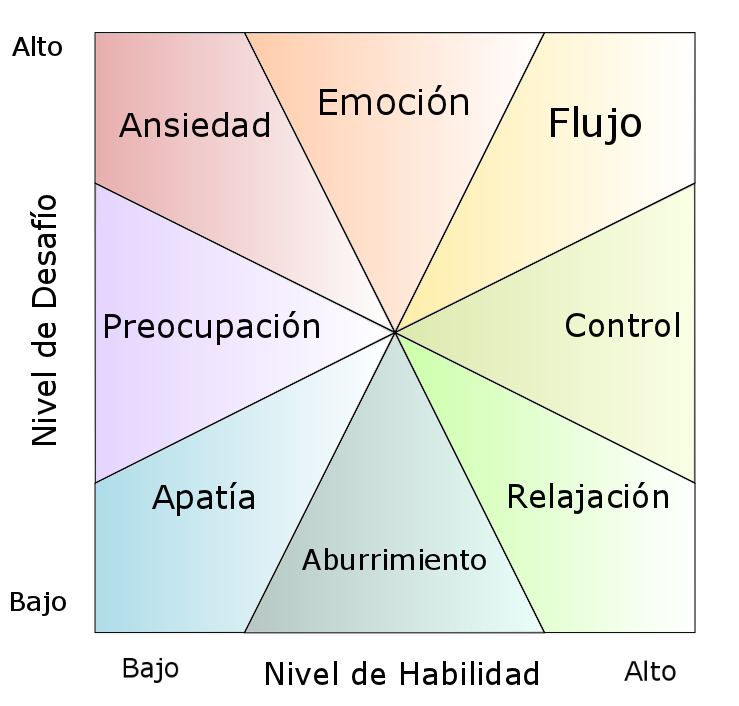
\includegraphics[scale=0.40]{img/Flujo.png}
\caption{Estados de la teoría del flujo.}
\label{fig::Flujo}
\small{Fuente: http://www.cluehuntervalencia.com}
\end{center}
\vspace{-0.5cm}
\end{figure}
\FloatBarrier

Csikszentmihalyi entrevistó a jugadores de ajedrez, artistas y deportistas, pero hoy en día, este fenómeno se produce con mucha frecuencia entre los gamers\footnote{Personas con una gran afición por los videojuegos}.
%
La distorsión de la percepción temporal que se produce en el estado de flujo es muy habitual.
%
¿Es posible establecer las condiciones necesarias en un sistema gamificado para que los jugadores entren en estado de flujo?


\subsubsection{Elementos de la Gamificación}

En esta sección vamos a ver los elementos y las herramientas generales con las que una persona puede diseñar una gamificación para un contexto específico.

Los elementos de la Gamificación son los elementos que podemos encontrar en los juegos, atendiendo a \cite{kwerb-pyramid} son: dinámicas, mecánicas y componentes.

\concept{Dinámicas} 
%
Las dinámicas son las estructuras implícitas del juego. 
%
Por ejemplo, las reglas serían una manifestación superficial de esa estructura implícita, pero las dinámicas también incluirían manifestaciones conceptuales como podrían ser las restricciones básicas de los juegos, por ejemplo, el respeto a las normas.
%
Por ejemplo, se considerarían dinámicas también las emociones, la narrativa, la progresión y las relaciones personales.\footnote{¿Debería incluir alguna definición o son suficientemente auto-explicativos?}

\concept{Mecánicas} Las mecánicas son los procesos que definen formalmente el contexto y que hacen avanzar la acción. 
%
Por ejemplo se considerarían mecánicas los retos, la suerte, la competición y la cooperación, el feedback, las recompensas, la adquisición de recursos, las transacciones y los estados de finalización\footnote{¿Debería incluir alguna definición o son suficientemente auto-explicativos?}.

\concept{Componentes} Los componentes son las instancias específicas de mecánicas y dinámicas. 
%
Serían componentes los logros, los avatares, los jefes finales\footnote{Batalla muy difícil que tiene lugar al final de cada nivel.}, los combates, el desbloqueo de contenido, los niveles, las misiones, los equipos, las posesiones y el grafo social.\footnote{¿Debería incluir alguna definición o son suficientemente auto-explicativos?}
%
Además, hay 3 componentes que merecen una mención específica: los puntos (points), las medallas (bdages) y los rankings (leaderboards), comúnmente llamados \gls{PBL}.


\paragraph{La gamificación es más que \gls{PBL}:} Es habitual confundir gamificación con un sistema de recompensas basado en \gls{PBL}. 
%
La gamificación trata de crear una experiencia centrada en el jugador. 
%
La implementación de un sistema de recompensas enfocado a realizar con eficiencia la función, dejando de lado la experiencia de los jugadores no puede ser considerada una gamificación y de hecho puede ser contraproducente.

Esta confusión es habitual porque estos tres componentes son fáciles de implementar y tienen varias funciones específicas que resultan muy útiles.
%
Los \textbf{puntos}, por ejemplo, otorgan un feedback acerca del rendimiento y el progreso, es una fuente de datos importante para el diseñador, pueden ligarse con recompensas y se pueden utilizar para determinar los estados de finalización.
%
Las \textbf{medallas} tienen una flexibilidad que permite definir el estilo de un jugador. 
%
Además, tienen un componente social muy importante, ya que muestran el estatus del jugador y son una representación de los logros conseguidos. 
%
También, algunos jugadores se sienten motivados a coleccionarlas.
%
Por último, los \textbf{rankings} o leaderboards crean un cierto sentido de competición, en el que los jugadores quieren ascender a puestos más altos del ranking, podría ser por el estatus que ofrecen esas posiciones.
%
Se ha estudiado que los leaderboards completos desmotivan al 80\% de las personas, debido a la gran brecha que se produce entre los primeros puestos y los últimos.
%
La aproximación más utilizada es diseñar leaderboards entre grupos más pequeños de jugadores, por ejemplo, entre los jugadores más cercanos con una puntuación cercana o con sus amigos.

\subsection{Algunos aspectos a tener en cuenta}

\subsubsection{Teoría de la motivación}
\label{SDT}
En la Psicología de la Motivación se ha establecido una diferencia entre 2 tipos de motivaciones\cite{SDT}:  \concept[Motivación\IS Intrínseca]{Motivación intrínseca} -- aquella que depende de los procesos cognitivos internos y está dirigida por el sentido de la autocompetencia, autonomía y relación -- y la \concept[Motivación\IS Extrínseca]{motivación extrínseca} -- aquella que depende de las recompensas que se puedan adquirir con la conducta realizada.
%
Por ejemplo, las actividades autotélicas, mencionadas en la teoría de flujo (ver \ref{autotel}), necesariamente conllevan una motivación intrínseca.
%
Además de esta diferencia se ha constatado que las conductas motivadas extrínsecamente dejan de realizarse cuando desaparece la fuente de motivación, incluso cuando en un momento anterior a la aparición de recompensas la conducta se llevara a cabo motivada intrínsecamente.

Es importante conocer esta diferencia a la hora de plantear el objetivo de nuestra gamificación. 
%
¿Interesa al diseñador crear un sistema sencillo basado en la motivación extrínseca de los jugadores o, por el contrario, diseñar un sistema más complejo que fomente y haga crecer la motivación intrínseca?



\subsubsection{Impacto de la competición en la motivación}

\label{PosiblesPeligros}
%
La competición es otra herramienta más a disposición del diseñador, pero es importante tener claro el resultado de algunas investigaciones.
%
Por ejempo, \cite{Crawford_CompetitionDef} señala que la competición puede centrar la atención en impedir que el contrincante venza en lugar de centrarse en mejorar y optimizar su propio desempeño.

Otro fenómeno estudiado por \cite{n-effect} es que el número de competidores y la motivación de los mismos mantienen una relación inversamente proporcional, es decir, cuantos más competidores, menor motivación.

Por último, un estudio llevado a cabo sobre la competición en la educación \cite{CompetitionInEd} constata que los premios para los ganadores deberían ser de poca importancia o incluso simbólicos para asegurar que el esfuerzo de los estudiantes es intrínseco y no está dirigido por la expetativa del premio.


\section{Educación gamificada}

Hasta ahora hemos estado tratando la Gamificación en términos generales, sin centrarnos específicamente en la educación. 
%
En esta sección trataremos de estudiar cómo se adapta esa teoría general al ecosistema de un aula.


\cite{lee2011gamification} sugieren que el sistema educativo ya contiene elementos de la gamificación, más concretamente \gls{PBL}, ya que los estudiantes realizan unos exámenes para obtener una calificación (puntos) y si se han obtenido más de 5 puntos, se obtiene la medalla de \textit{aprobado}.
%
Incluso, se puede obtener la medalla de \textit{mención de honor} en la evaluación final.
%
Además, encubiertamente se forma un leaderboard, ya que los alumnos tienen claro quienes son los mejores y los peores alumnos (en términos de calificaciones obtenidas).
%
Sin embargo, estos elementos no implican necesariamente motivación por parte de los alumnos.
%
Diseñar una gamificación en un aula puede motivar a los estudiantes, ofrecer a los profesores mejores herramientas para guiar y recompensar a sus estudiantes y enseñar a los estudiantes que la educación puede ser una experiencia divertida \cite{lee2011gamification}.

Es importante tener en cuenta que la gamificación en educación no debería basarse en una motivación extrínseca, sino fomentar la motivación intrínseca. 
%
De esta manera, los estudiantes podrán desarrollar una mayor capacidad para valorar el aprendizaje y cuando avancen a lo largo del sistema educativo sean capaces de aprovechar contextos educativos no gamificados. 

En la sección \ref{sec:EstadoEducacionMates} se comentó la existencia de un círculo vicioso (ver figura \ref{fig::circuloVicioso}) y que la variable más influyente en el rechazo hacia las Matemáticas en España es la percepción de la materia como aburrida o divertida.
%
Esperamos que, tras lo expuesto, el lector esté de acuerdo en que la Gamificación puede ayudar a modificar esa percepción aprovechando que existen tareas difíciles y divertidas (ver \ref{kindsoffun}) además de romper el círculo vicioso por 2 extremos diametralmente opuestos: aburrimiento y desmotivación.


